This chapter explains the mapping process of HTSLAM. First, the
technique used for building local maps is presented in
section~\ref{sec:local_mapping}. Section~\ref{sec:topological_pose}
deals with the problem of tracking of robot pose in the topological
structure of the HTSLAM map. The procedure for starting a new local
map is described in section~\ref{sec:starting_new_map}.
Section~\ref{sec:revisiting} explains how revisiting previously
mapped regions is handled in HTSLAM.

\section{Initialisation}

It is generally assumed in the SLAM literature that a robot starts
with absolutely no knowledge of the environment. The robot does not
know how many landmarks there are or where they are located: its map
is initially empty. Similarly, in HTSLAM the initial map contains just
one region and an empty map.


\section{Local Mapping Procedure}
\label{sec:local_mapping}

\SILENT{
\begin{itemize}
\item Underlying mapping module: FastSLAM
\item Modifications to FastSLAM: particles can be in different map
  frames, time holes and teleportations.
\item Why is it better than EKF: faster, multi-hype, better
  uncertainty modelling.
\item Summary of operation: how we start, state variables/data,
  multiple hypotheses.
\end{itemize}
}

%%% \subsection{ Rao-Blackwellised Particle Filter}
%%% 
%%% \SILENT{
%%% 1. Faster: No need for cross-correlation between landmarks is a very
%%% big advantage, since updates to the cross-correlation matrix have a
%%% computational complexity of $O(N^3)$ ($O(N^4)$ using the trivial
%%% approach). In FastSLAM each landmark is updated independently, and
%%% only when it is observed. The computational complexity of the update
%%% step depends only on the number of particles. The data association
%%% though depends on the number of landmarks as well as on the number of
%%% particles. Overall FastSLAM computational complexity is linear in the
%%% number of particles $M$ and logarithmic in the number of landmarks
%%% $O(M \log N)$.
%%% 
%%% 2. Intrinsic support for multiple hypotheses - makes it really easy
%%% to extend to multiple local maps, very natural integration into our
%%% global map structure.
%%% }
%%% 
%%% The main advantage of using Rao-Blackwellised particle filters for mapping
%%% is the fact that they are fast, hence FastSLAM. The computational
%%% complexity of the FastSLAM approach is $O(M \log N)$, $N$ being the
%%% number of landmarks, and $M$ the number of particles. Storage
%%% requirements for FastSLAM is $O(M N \log N)$. In contrast EKF memory
%%% and computational requirements are $O(N^2)$, due to the fact that the
%%% EKF maintains full cross correlation matrix between all landmarks and
%%% robot pose. In HTSLAM the size of the environment is limited, hence
%%% scalability of the local mapping algorithm is not that
%%% important. FastSLAM has other advantages though.
%%% 
%%% Another advantage of the particle filter approach over the EKF is its
%%% superior model of uncertainty. The EKF linearises the motion model so
%%% that the posterior distribution over robot pose is Gaussian. FastSLAM
%%% samples directly from the motion model. More importantly, FastSLAM can
%%% capture the uncertainty of the data association decisions, something
%%% that is impossible with an EKF.  This is especially advantageous when the
%%% environment is cluttered. It is well known that the EKF is very
%%% sensitive to errors in data association decisions
%%% \cite{neira01:_data_assoc_stoch_mappin_using}.  FastSLAM provides a
%%% more robust solution to mapping with unknown data association.
%%% 
%%% Particle filtering based approaches can incorporate negative information
%%% (i.e. expect to see landmark but don not) into the computation of the
%%% likelihood of the path. While negative information is not used in this
%%% implementation, it can provide a wealth of useful information in some
%%% environments.
%%% 

\subsection{Modifications to the Rao-Blackwellised Particle Filter}

%time holes, teleportations, mainly affects the notation,
%implementation-wise the same as normal FastSLAM.

In this work mapping within a local map is performed using
FastSLAM. However, due to the nature of HTSLAM, some modifications have
to be made to the original FastSLAM algorithm. The changes affect
mainly notation; modifications to the actual implementation of a local
map building algorithm are minimal.  Unlike the global approach, in
HTSLAM each local map is updated only when the robot is within the
region of the map. A local map at time $k$ is conditioned on a subset
of all observations and control inputs. \Zall{k}{} denotes a set of
all observations up to time $k$, \Zall{k}{a} is a subset of \Zall{k}{}
and contains only observations relevant to the region $a$ (i.e. taken
when the robot was in the region $a$). Similarly, \Uall{k}{} is a set
of all control inputs issued up to time $k$, and \Uall{k}{a} is a
subset relevant to region $a$. The set \Xall{k}{}{a} denotes all robot
poses within a local map $a$ from time $0$ up to time $k$.

In global SLAM the pose of the robot is continuously being tracked by
the filter. The set of all observations and control inputs up to time
$k$ and an initial pose at time 0 is sufficient to estimate robot pose
at time $k$. In HTSLAM the robot disappears from the local map at some
point, to reappear later in a completely different spot. To a mapping
module this ``teleportation'' of the robot from one spot at time $k_1$
to another at time $k_2$ appears as a special kind of control input
\Teleport{k_1}, where the robot position at time $k_2$ is taken to be 

$$
\x{k_2}{}{a} \sample{}{} \prob{\x{k_1}{}{a} | \Teleport{k_1}}
$$

The set of all such teleportations is denoted \TeleportAll{k}{a}. For
each local map HTSLAM estimates the probability density

$$
\prob{\map{k}{}{a},\Xall{k}{}{a} | 
\Zall{k}{a},\Uall{k}{a},\TeleportAll{k}{a},\x{k_0}{}{a}},
$$
where \map{k}{}{a} is a map of the region $a$ and \x{k_0}{}{a} is an
arbitrary initial robot pose (typically at the origin).




\section{Monitoring Robot Location in the Topological Map}
\label{sec:topological_pose}

At every point in time the robot maintains a map of neighbourhood
region. A neighbourhood consists of the current map and a set of maps
that are close to a current one in a topological and Cartesian sense.
The neighbourhood region is a union of the current map region and
projections of neighbouring regions onto the current coordinate frame.
Two regions are not considered neighbours if their relative pose
uncertainty is too high.

\begin{figure}
\begin{center}
\subfigure[Mapping region {\bf A}]{
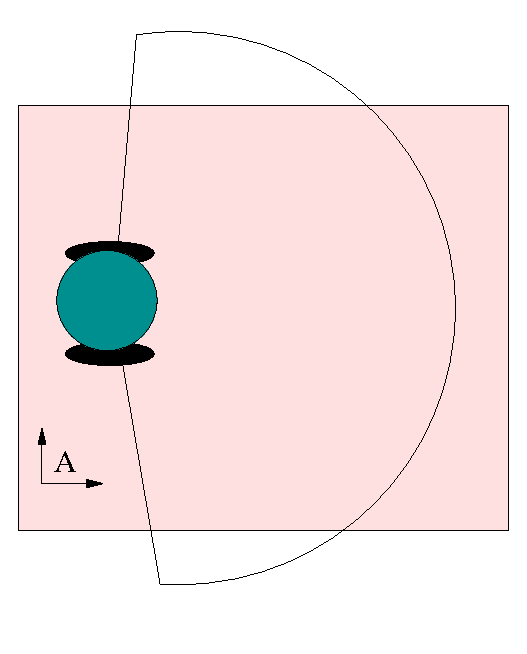
\includegraphics[height=3cm]{Pics/fig_transition1}
\label{fig:StartNewa}
}\quad \quad \quad
\subfigure[Entering Unexplored Area (region {\bf B})]{
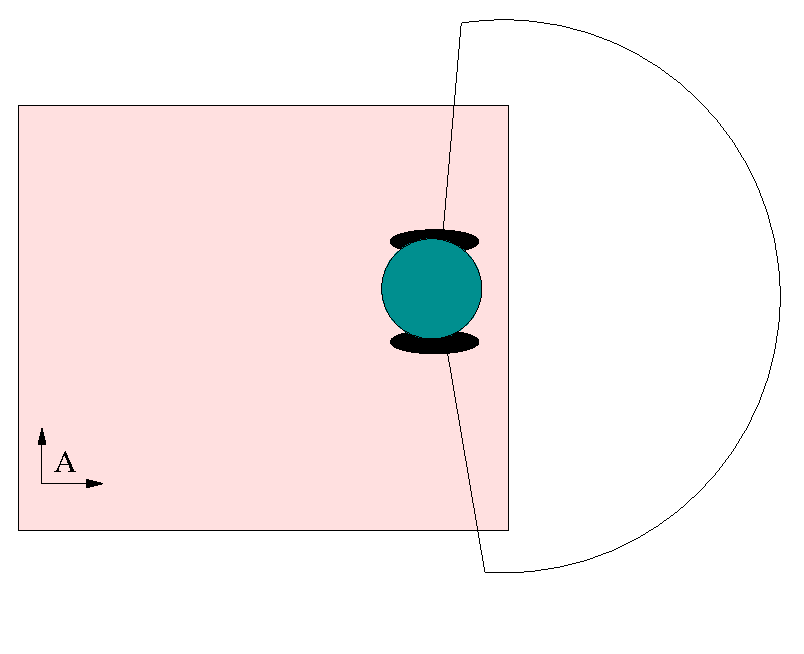
\includegraphics[height=3cm]{Pics/fig_transition2}
\label{fig:StartNewb}
}\quad
\subfigure[Coming Back to region {\bf A}]{
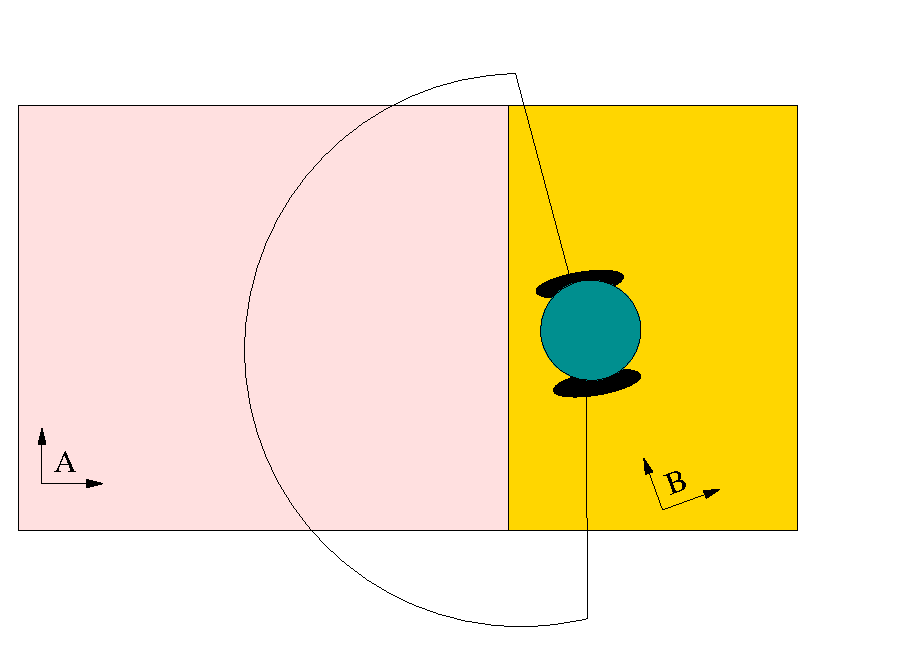
\includegraphics[height=3cm]{Pics/fig_transition3}
\label{fig:StartNewc}
}
\end{center}
\caption[Map regions used for triggering transition events]
{The overlap between the sensor range and the area of the local 
 map is used to decide when to start a new map or transfer to a 
 neighbouring region.}
\label{fig:StartNew}
\end{figure}

The robot constantly checks how much of the sensor field of view falls
within the current region (see \refFigure{fig:StartNew}), and how much
falls in the neighbouring regions. When the robot detects that one of
the neighbouring regions has a significantly large overlap with the
sensor field of view, it switches to that region. The goal is to
maximise the proportion of observations that match to an existing map.
If one assumes uniform distribution of landmarks in the environment
and uniform detection rates for a sensor view (i.e. a landmark
straight ahead is as easily detectable as one on the robot's left),
then this approach actually maximises the number of re-observed
landmarks. In the real world landmarks are not distributed uniformly,
and the detection rates for different views of a landmark are
different. This approach nevertheless provides a good, computationaly
inexpensive measure for determining map transitions.

A sensor view based approach also makes the decision to start a new
map trivial. If no region overlaps sufficiently with the sensor field
of view, the robot assumes it is entering an unexplored area and
initiates a new map. In order to avoid oscillations between two
regions when the robot is near the boundary, thresholds are set to
slightly favour staying in the current region.


\section{Starting a New Local Map}
\label{sec:starting_new_map}
%How it is done.
%\begin{enumerate}
%\item Finalise current map.
%\item Add new node and link to the map graph.
%\item Initialise particles - empty map, 0 pose.
%\item Compute initial area.
%\item Subtract ``neighbours''.
%\end{enumerate}


The pose of a robot is represented by a set of particles: at any time
instant HTSLAM maintains a set of path particles, and the
corresponding maps conditioned on the path. When a new map is started
the relative pose of the current and new map reference frames is
different for every particle. Since the pose of the robot in the new
map is known exactly (and so is equal for every particle), it is
possible to compute the relative transformation between the two maps
for every particle. A set of particles is treated as a sample from
the distribution $\prob{\tr{}{A}{B},\mapA}$.  The new empty map that
is created is independent of the previous path of the robot, hence

$$
 \prob{\mapA,\tr{}{A}{B},\mapB} = \prob{\mapA,\tr{}{A}{B}}\prob{\mapB}.
$$

Furthermore, tuple $(\mapA, \tr{}{A}{B})$ is actually a single variable.
Since the map is conditioned on the path of the particle, there exists a
one to one non-random relationship between the transition and map $A$,
that is $\tr{}{A}{B} = f(\mapA)$. Therefore

$$
\prob{\mapA,\tr{}{A}{B},\mapB} \equiv \prob{\mapA,\mapB}.
$$

At the time when \mapB is started $\prob{\mapA,\mapB}$ is assumed to
be a discrete uniform distribution - a pair of map instances from
\mapA and \mapB is considered to be equally likely. This is due to the
fact that \mapB is empty, and so any sample from \mapB is equally
``compatible'' with any sample from \mapA. As \mapB is explored, more
information, that can be used to evaluate the relative compatibility
of the $(\mapA,\mapB)$ sample becomes available. If, for example, a
set of landmarks appears in both \mapA and \mapB, and their
correspondence is known, one can evaluate the likelihood of the map
pair using covariance intersection \cite{cov_intersection} of the
common landmarks. However there is no need to continuously update the
transition distribution; it is assumed to be unchanged until it is
time to sample from it. The only information that needs to be stored
at the time of creating a transition is a mapping $\mapA \Rightarrow
\tr{}{A}{B}$.


The process of creating new map as follows:

\begin{enumerate}

\item A new node is added to the graph, and is connected to the
  current map.

\item The current reference frame is set to that of the new node.

\item The pose of all particles is set to some initial value (0),
  their maps are set to empty, and the mapping process is restarted.

\end{enumerate}

As the robot continues mapping the new region, any error in the map
and robot pose estimate remains conditionally independent of errors
in any previous maps. This independence remains until the region is
revisited.


\section{Switching Maps - Revisiting}
\label{sec:revisiting}
%\begin{itemize}
%   \item How we decide to transfer to a different map.
%   \item What happens when we do.
%   \item Describe difference between traversing the link first
%        time and thereafter.
%\end{itemize}

When the robot detects that there is a significant overlap between one
of the neighbouring regions and the sensor field of view, it switches
to the corresponding local map. Typically, the neighbouring region
will be adjacent to the current region, however two regions that are
separated by several links in the graph can also be considered
neighbours if the compound coordinate transformation from one to the
other is sufficiently certain.  In the case when the regions are not
directly connected, the transition is performed along the shortest
path between the two regions and is equivalent to performing several
transitions sequentially. The procedure for computing the shortest
path between two local maps is discussed in the chapter on loop
closing (Chapter~\ref{chpt:LoopClosing}).

Consider the transition under the assumption that the two regions are
adjacent. Let $A$ be the region mapped first, and $B$ the region
created subsequently. As described previously
(Chapter~\ref{chpt:MapStructure}), each transition maintains joint
probabilities that capture the three-way relationship of the two maps
joined by the transition and their relative pose. It is therefore
possible to sample a map-transition-map triple $\{
{\mapA,\tr{}{A}{B},\mapB} \} \sim \prob{\mapA,\tr{}{A}{B},\mapB} $.
 

\begin{figure}
\begin{center}
\subfigure[Path in region {\bf A}.]{
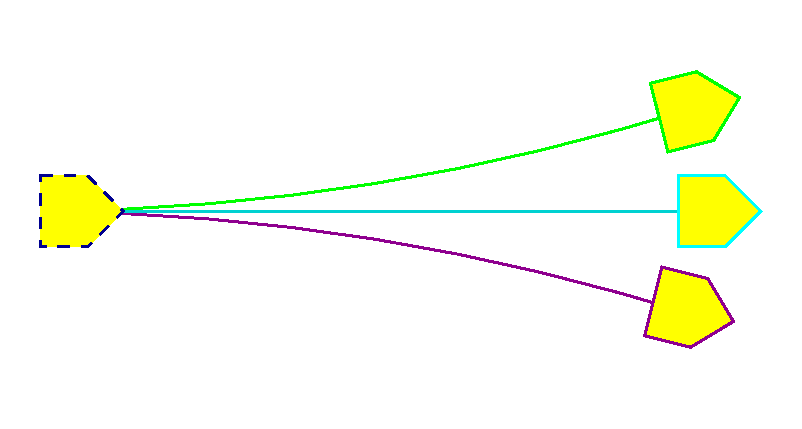
\includegraphics[height=2cm]{Pics/fig_revisit1}
\label{fig:MappingExampleA}
 }
 \subfigure[Path in region {\bf B}.]{
 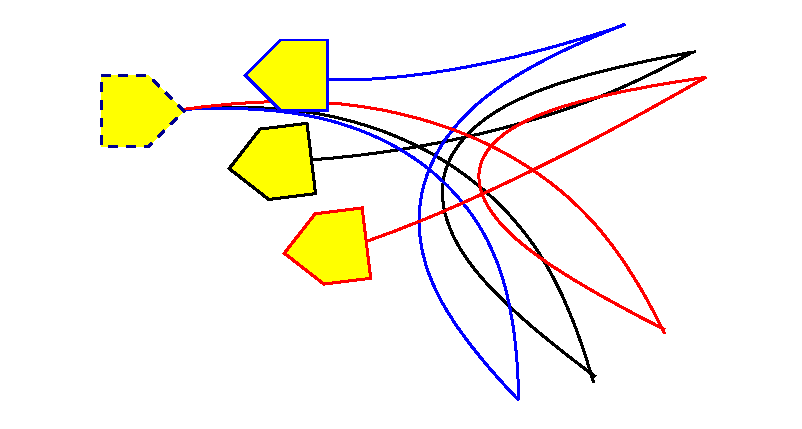
\includegraphics[height=2cm]{Pics/fig_revisit2}
 \label{fig:MappingExampleB}
 }\\
 \subfigure[Combined paths.]{
 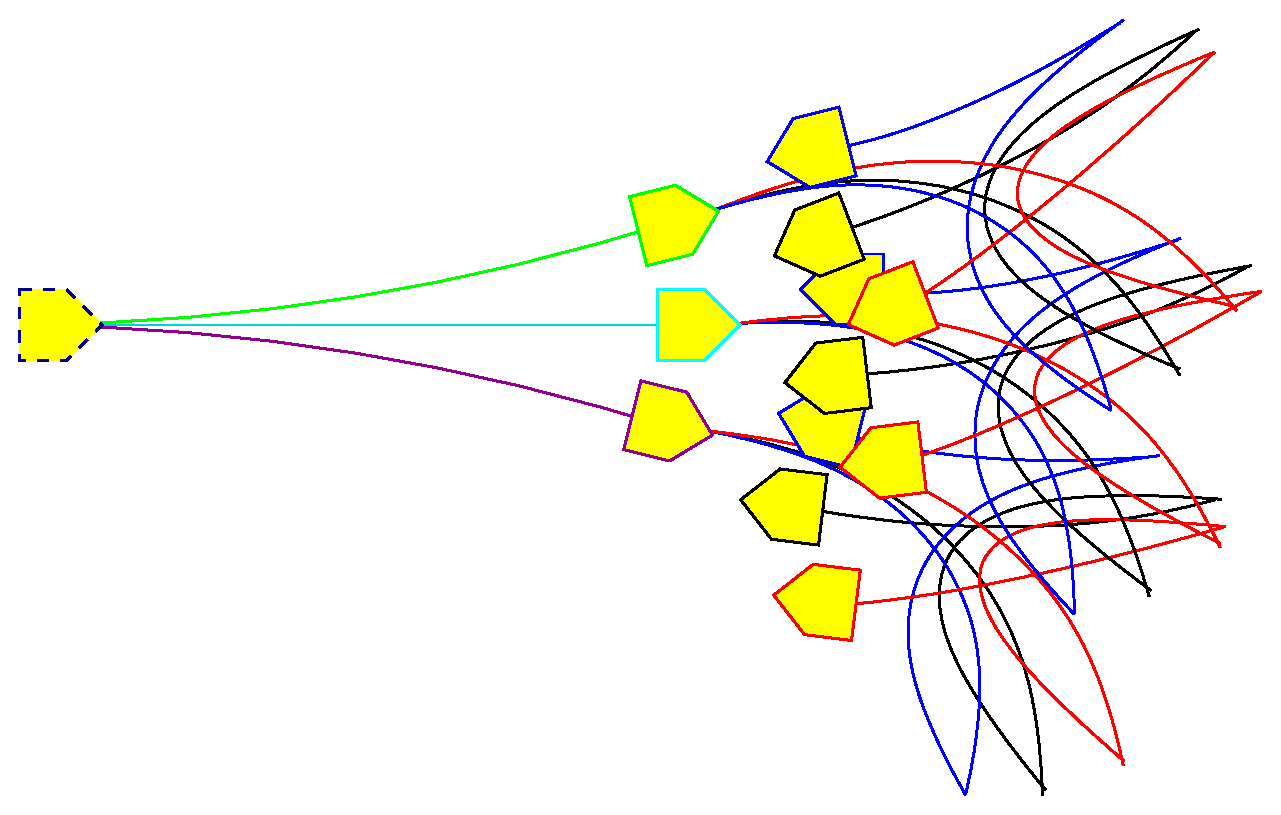
\includegraphics[width=6cm]{Pics/fig_revisit3}
 \label{fig:MappingExampleC}
 }
 \subfigure[Sampled paths.]{
 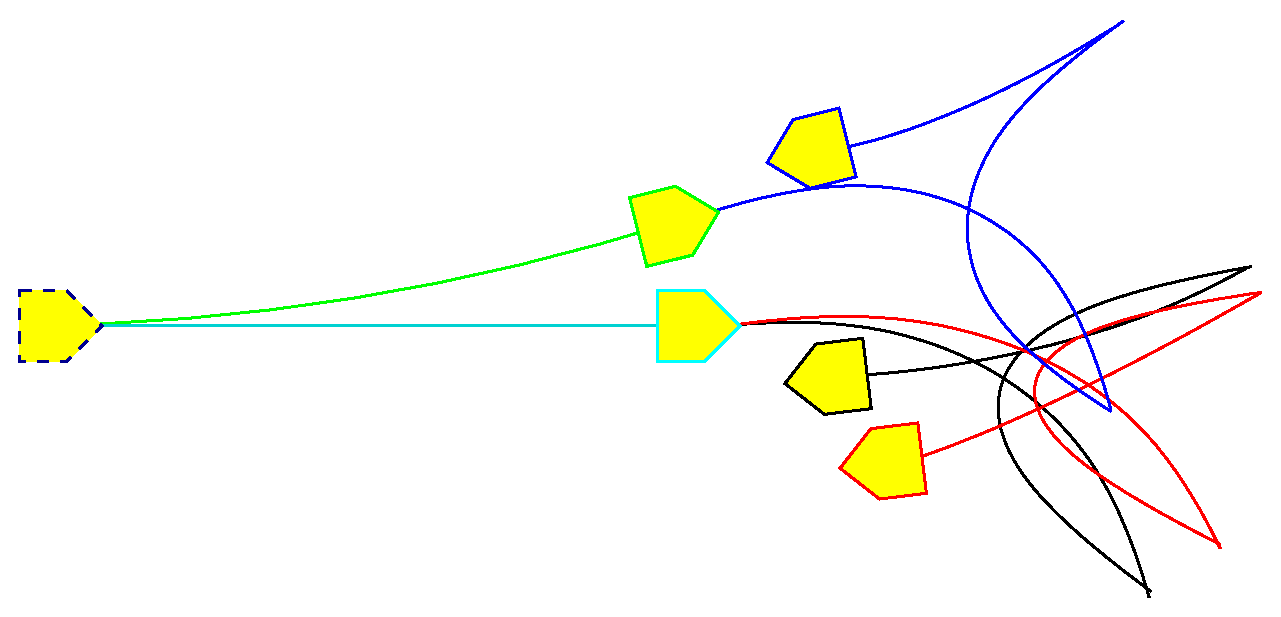
\includegraphics[width=6cm]{Pics/fig_revisit4}
 \label{fig:MappingExampleD}
 }
 \end{center}
 \caption{Example: revisiting map region.}
 \label{fig:MappingExample}
\end{figure}



It is best to describe the process of transition from one map to
another with an example, referring to
\refFigure{fig:MappingExample}. The robot has a car-like driving
system and lives on a plane. Three particles are used to approximate
the robot's motion. The robot starts in region $A$ and travels some
distance forward, taking observations. Some time later the robot
reaches the boundary of region $A$ and starts a new map $B$. Again
three particles are used to model the uncertainty of the robot's path
in map $B$. After performing a three point turn the robot returns to
region $A$. At this point there are 9 possible paths the robot could
have taken. These paths are illustrated in
\refFigure{fig:MappingExampleC}. By starting a new map $B$, HTSLAM
effectively conserves the uncertainty at that time instant. Now, when
the robot is returning to the region $A$ there are more possible paths
to consider. More hypotheses are beneficial. The number of hypotheses
is akin to resolution in images - more hypotheses provide a clearer
picture of the observed uncertainty. HTSLAM uses only 3 particles for
mapping but has 9 possible paths. A global mapping approach would have
had to use 9 particles (that is $N^2$) to get the same ``resolution''
on the uncertainty. While having higher resolution is desirable,
computational resources are limited. Therefore in this example only 3
paths have to be sampled.

One can assume that all paths are equally likely and sample
appropriately. This approach is, however, wasteful. If the two maps
share common landmarks, it should be possible to evaluate each path
based on some map overlap criteria that approximate
$\prob{\mapA,\mapB}$.

Alternatively one can use some form of adaptive particle filter
\cite{KLDSampling} that adjusts the number of particles
based on the spatial uncertainty in the robot's pose. In the case of a
transition from one map to another, the uncertainty of the robot's
location increases and hence the number of particles would be
temporarily increased. After some observations of map $A$, bad paths
would be pruned out through the process of re-sampling. 

%% \NOTE{I reckon
%% this approach is a better one. It is however not very clear, what will
%% happen when running multiple hypotheses (loop closing). I know it have
%% been done for localisation, but can not find any references for SLAM.}

Once the robot transfers from $B$ to $A$ the two maps are no longer
independent. Any further update to map $A$ will depend on the pose of
the robot in map $A$. Robot pose in map $A$ depends on the transition
and on robot pose in map $B$ at the time of transition, which in turn
depends on map $B$. All three variables, map $A$, map $B$ and the
transition between them are therefore dependent variables. This
dependency is represented in the HTSLAM structure by a sample from the
$\prob{\mapA,\tr{}{A}{B},\mapB}$.

In practice this means that each particle now knows which map to
update in $A$ and in $B$, and which transition to use when
transferring from one to the other \SILENT{need to be more clear about
the samples from map A,B}. From that point onwards no sampling will be required
when transferring from $A$ to $B$ and back. If the robot continues
operating only within these two maps, the mapping process will be
equivalent to a normal FastSLAM, except that the environment is split
into regions of bounded size, and hence computation requirements are
bounded.

Due to the process of re-sampling, the overall uncertainty in the
transition between maps $A$ and $B$ will decrease over time, as more
observations become available. This is due to the fact that particles
that ended up with ``bad'' transition hypotheses won't match
observations to the map as well as the ones with ``good'' transition
hypotheses, and will be pruned out during the re-sampling stages of
the particle filter. While this is generally a good thing, there is a
drawback: the particle deprivation problem. Since there is no process in
place that will introduce new particles to the transition, over time
the transition estimate will collapse to just a few or even one
particle. 

%\NOTE{Why is it a problem, when is it not a problem. What
%can be done about it. }

If the robot starts a new region $C$ and then returns to
region $A$, a similar process of sampling will occur. This time,
however, every map in $A$ is linked to a map in $B$ and to the
transition between regions $A$ and $B$.


% LocalWords:  FastSLAM Montemerlo Thrun Kalman EKF Submap observability endfor
% LocalWords:  Bayes endif odometry ms XR holonomic Nieto HTSLAM teleportations
% LocalWords:  teleportation Rao Blackwellised
